\documentclass{article}

%%%%%%%%PACKAGES%%%%%%%%
\usepackage{amsmath} 
\usepackage{amsfonts}
\usepackage{siunitx} 
\usepackage{physics}
\usepackage{geometry}
\usepackage{graphicx}
\usepackage{float}
\usepackage{hyperref}
\usepackage{url}
\geometry{margin=1in} 

\newtheorem{definition}{Definition}

%%%%%%%%TITLE%%%%%%%%
\title{Notes on Higher-Form Symmetries}
\author{Gabriel C. Magalhães\footnote{gabriel.capelini@uel.br}}
\date{2025}

\begin{document}
\maketitle

\begin{abstract}
These notes present  my current understanding of higher-form symmetries and are intended for pedagogical purposes. They are continuously updated as I learn more about the subject and are based on the references listed below.
\end{abstract}

\tableofcontents
\pagebreak

\section{Introduction}
Higher-form symmetries generalize conventional global symmetries by acting on extended operators, such as line or surface operators, rather than local, point-like ones. These symmetries are characterized by topological symmetry operators, and their action is defined via the linking of the manifold supporting the symmetry operator with the manifold supporting the charged operator. A key consequence is that the associated conserved currents become higher-degree differential forms, in contrast to the standard 1-form currents of ordinary symmetries.

To build intuition, we will first revisit the topological interpretation of ordinary symmetry operators before extending these ideas to the higher-form case.



\section{Symmetry Operators as Topological Operators}
In terms of differential forms, the conservation law is written as
\begin{equation}
	d\star j=0,
\end{equation}
where $j$ is the current 1-form and $\star:\Lambda^p\to \Lambda^{D-p}$   is the Hodge star map that take a p-form and associates it to a $(D-p)$-form. The conserved current is defined as
\begin{equation}
	Q\equiv\int d^{D-1}x\;j^0.
\end{equation}
In terms of differential forms, we may write as
\begin{equation}
	Q=\int_{\Sigma_{D-1}}\star j,
\end{equation}
where $\Sigma_{D-1}$  is a $(D-1)$-dimensional manifold. We say then that those charges are integrated over a codimension-1 manifold, which is a submanifold of some $D$-dimensional manifold.  To understand how these operators act over the fields, we will make use of the Ward identity,
\begin{equation}
	\partial_\mu\langle j^\mu(x)\phi(y)\rangle=-i\delta^{(D)}(x-y)\langle\delta\phi(y)\rangle.
\end{equation}
Integrating over a $D$-dimensional manifold $\Omega$  with boundary $\Sigma_{D-1}$, the left-hand side becomes
\begin{equation}
	\int_{\Omega}d\langle\star j\phi(y)\rangle=\int_{\Sigma_{D-1}}\langle\star j\phi(y)\rangle=\langle Q(\Sigma_{D-1})\phi(y)\rangle,
\end{equation}
where we have used Stokes theorem. For the right-hand side, we have
\begin{equation}
	-i\int_{\Omega}d^Dx\;\delta^{(D)}(x-y)\langle\delta\phi(y)\rangle,
\end{equation}
where we identify,
\begin{equation}
	\int_{\Omega}d^Dx\;\delta^{(D)}(x-y)=\begin{cases}0,\quad y\in\Omega\\1,\quad y\not\in\Omega\end{cases}
\end{equation}
as the linking between the point $y$ and the manifold $\Omega$. Thus we call  
\begin{equation}
	\int_{\Omega}d^Dx\;\delta^{(D)}(x-y)\equiv \text{Link}(\Sigma_{D-1},y).
\end{equation}
Hence
\begin{equation}
	\langle Q(\Sigma_{D-1})\phi(y)\rangle=-i\text{Link}(\Sigma_{D-1},y)\langle\delta\phi(y)\rangle.
\end{equation}
What this expression is telling us is that the charge acts on the local field, and it only have non-vanishing action if the point where the local operator is defined links with the manifold where the charge is defined. The link is unaffected by deformations, as longs as they do not cross the point $y$.  To see this, suppose that we perform a deformation of the type $\Sigma'=\Sigma+\Sigma_0$, $y\not\in\Omega_0.$ Then 
\begin{equation}
	Q(\Sigma+\partial\Omega_0)=\int_{\Omega\cup\Omega_0}\langle d\star j\phi(y)\rangle=\int_{\Omega}\langle d\star j\phi(y)\rangle+\int_{\Sigma_0}\langle d\star j\phi(y)\rangle.
\end{equation}
Since $\text{Link}(\Sigma_0,y)=0,$ then
\begin{equation}
	Q(\Sigma+\partial\Omega_0)=\int_{\Omega}\langle d\star j\phi(y)\rangle=Q(\Sigma).
\end{equation}
That is the reason why we call these \textit{topological operators}. The unitary operator is defined by taking the exponential of the conserved charge,
\begin{equation}
	U(g,\Sigma_{D-1})=\exp(i\alpha_aQ_a)=\exp\left(i\alpha\int\star j\right),
\end{equation}
where $g\in G$  is an element of some group $G$ and $\alpha_a$ are the parameters of the transformation. In the case of  $U(1)$  we have $g=e^{i\alpha}$.  We say then that this is a topological codimension-1 operator. 

In terms of the unitary operator, the action over the local operators is given by
\begin{equation}
	\langle U(g,\Sigma_{D-1})\mathcal{O}(x)\rangle=R(g)\langle\mathcal{O}'(x)\rangle,
\end{equation}
where $R(g)$ is the representation under which the operator $\mathcal{O}(x)$ transform. 
Since operators are defined over a Hilbert space at a constant time, we cannot compare operators at different times. Since the manifold $\Sigma_{D-1}$ need not to be necessarily a spatial slice for general topological operators, the expression only makes sense inside correlation functions, where we can compare operators at different spacetime points without problem. What is happening diagrammatically is shown below. 

Let   $U(S^{D-1})$ be an operator defined over a $(D-1)$-sphere.  As we have seen, these operators act over local operators $\mathcal{O}(x)$ and transforms them into another operator $\mathcal{O}'(x)$  as shown in the figure
\begin{figure}[H]
\centering
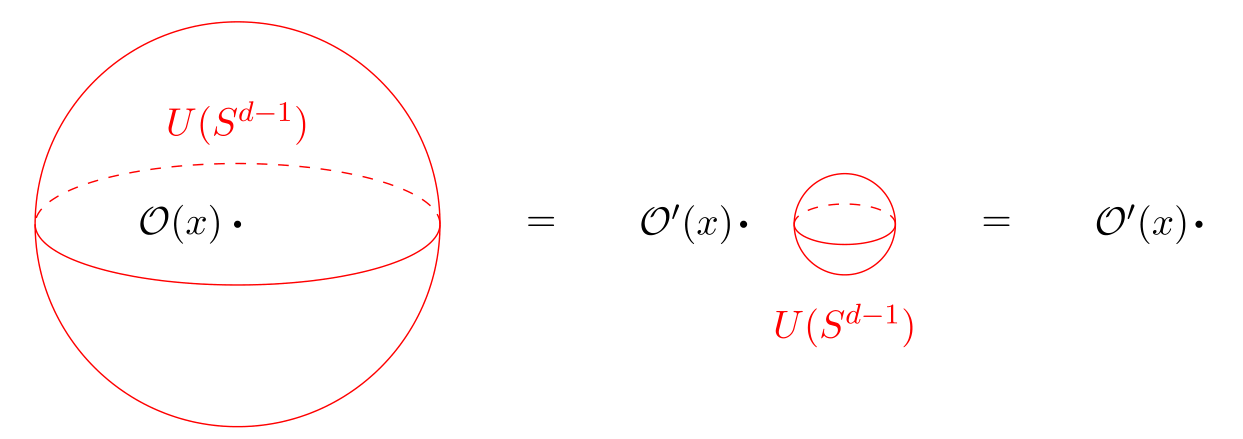
\includegraphics[scale=0.3]{figures/linking.png}
\caption{Taken from \cite{Bhardwaj}.}
\end{figure}
The operator $U(S^{D-1})$ links with $\mathcal{O}(x)$ then we deform it until it no longer links. Then we can deform $S^{D-1}$ to a point and the reminiscent operator is what we call $\mathcal{O}'(x).$ 
\subsection{0-form Groups}
We define the 0-form group $G^{0}$ to be the group composite of the elements $g$ that parametrizes the operator $U_g.$

The composition of two topological operators are given by the composition law of the group
\begin{equation}
	\langle U_g(\Sigma_{D-1})U_{g'}(\Sigma_{D-1})\rangle=\langle U_{gg'}(\Sigma_{D-1})\rangle.
\end{equation}
Thus, inserting the composition of topological operators into these correlation functions is equivalent to insert one topological operator with the composition of the elements. This is called the fusion rule,
\begin{equation}
	U_g\otimes U_{g'}=U_{gg'}.
\end{equation}
From now on, we will drop the correlation function notation but it is to be understood that it is there unless it said the contrary.  We now give a more formal definition of a 0-form symmetry. 

\begin{definition}
	A 0-form symmetry is a codimension-1 operator that is topological and invertible.
\end{definition}
Topological means that
\begin{equation}
	U_g(\Sigma_{D-1})=U_g(\Sigma'_{D-1}),
\end{equation}
if we can deform $\Sigma_{D-1}$ continuously into $\Sigma'_{D-1}.$  The invertibility property follows from the composition rule 
\begin{equation}
	U_g(\Sigma_{D-1})U^{-1}_g(\Sigma_{D-1})=1.
\end{equation}
We may now understand how the topological operator computes the charge of the local operators. Note that for an operator $\mathcal{O}(x) $ with charge $q$, the Ward identity becomes (without the correlators) 
\begin{equation}
	\partial_\mu j^\mu(y)\mathcal{O}(y)=q\delta^{D}(x-y)\mathcal{O}(y),
\end{equation}
where it was used the fact that $\mathcal{O}(x)\to e^{i\alpha q}\mathcal{O}(x)$. In terms of differential forms, 
\begin{equation}
	(d\star j)\mathcal{O}(x)=q\delta^{D}(x)\mathcal{O}(x),
\end{equation}
where $\delta^D(x)$ is the Poincaré dual of $\delta^D(x-y)$. Thus for an operator $U(S^{D-1})$ acting over a local operator $\mathcal{O}(x), $ we have 
\begin{equation}
 \begin{split}
 	U(S^{D-1})\mathcal{O}(x)&=\exp\left(i\alpha\int_{S^{D-1}}\star j\right)\mathcal{O}(x)\\&=\exp\left(i\alpha\int_{\Omega_D}d\star j\right)\mathcal{O}(x)\\&=\exp\left(i\alpha\int_{\Omega_D}q\delta^D(x)\right)\mathcal O(x)\\&=\exp(i\alpha q)\mathcal{O}(x),
 \end{split}
\end{equation}
where $\Omega_D$ is some $D$-dimensional manifold with boundary $S^{D-1}$. 
\section{Higher-Form Symmetries}
With our formal definition, it is easy to generalize the idea to higher-form symmetries. 

\begin{definition}
	A p-form symmetry is a codimension-$(p+1)$ operator that is topological and invertible. 
\end{definition}
Let’s see why it must be a codimension-$(p+1)$ operator. Consider the variation of the action when we take the parameter of the symmetry to be local,
\begin{equation}
	\delta S=\int d^4x\;j_\mu\partial^\mu\Lambda.
\end{equation}
For a $D$-dimensional space and in the language of differential forms, this equation becomes 
\begin{equation}
	\delta S=\int\star j\wedge d\Lambda.
\end{equation}
Consider that $\Lambda$  is a p-form, consequently $d\Lambda$ will be a $(p+1)$-form. Then, in order to match the dimension of the spacetime, $\star j$ must be a $(D-p-1)$-form. This implies that the conserved charge will be 
\begin{equation}
	Q=\int_{\Sigma_{D-p-1}} \star j,
\end{equation}
and the unitary operator is defined as before
\begin{equation}
	U_g(\Sigma_{D-p-1})=\exp\left(i\alpha\int_{\Sigma_{D-p-1}}\star j\right),
\end{equation}
where now this is understood as a codimension-($D-p-1$) operator.
We now must look at which objects are charged under those symmetries, that is, which objects the $p$-form operators act on.

The same rules from before apply here. There is an inverse operator
\begin{equation}
	U_g(\Sigma_{D-p-1})U_g^{-1}(\Sigma_{D-p-1})=1.
\end{equation}
The group of p-form symmetries $G^{p}$  consists of the elements that parametrize the operator $U_g(\Sigma_{D-p-1}).$ Just as before, the composition of those operators is given by  
\begin{equation}
	U_g(\Sigma_{D-p-1})U_{g'}(\Sigma_{D-p-1})=U_{gg'}(\Sigma_{D-p-1}),
\end{equation}
which is denoted the fusion rule 
\begin{equation}
	U_g\otimes U_{g'}=U_{gg'}.
\end{equation}
Moreover, the $p$-form symmetry group is abelian for $p\ge 1.$ This follows because we can deform an operator over another without ever crossing them. 

The “usual” symmetries are now understood as 0-form symmetries, because the parameter of the transformation is a closed 0-form. The 0-form symmetries act over local operators, whose are supported on 0-dimensional regions. This is something we understand from standard QFT. We say then that the local operators are charged under the 0-form symmetry. We now wish to understand which objects are charged under p-form symmetries. It is straightforward to note that for $p\geq1,$ the $p$-form symmetry will never act over a local operator because we can always deform the operator in a way that it doesn’t intersect with the point. Therefore, the $p$-form symmetry acts over objects that have a dimension $q\geq p$.
\subsection*{Case $q=p$}
For this case, we define an operator $U_g(\Sigma_{D-p-1})$ over a $(D-p-1)$-dimensional manifold that links with some operator  $\mathcal{O}(M_p)$ defined over a $p$-dimensional manifold. Then we deform $U_g(\Sigma_{D-p-1})$  over $\mathcal{O}(M_p)$, leaving behind a local operator $\mathcal{O}(x)$ as before. We can assume that the only local operators that can be inserted along the manifold $M_p$ are multiples of the local identity operator. Thus, we may say that these multiples are complex numbers $\phi(g)$,  
$$
\phi(g)\in \mathbb{C}^{\times},\quad \mathbb{C}^{\times}\equiv \mathbb{C}\backslash\{\ 0 \}.
$$
The action of the operator $U_g$ over $\mathcal{O}$ is represented below. 
\begin{figure}[H]
	\centering
	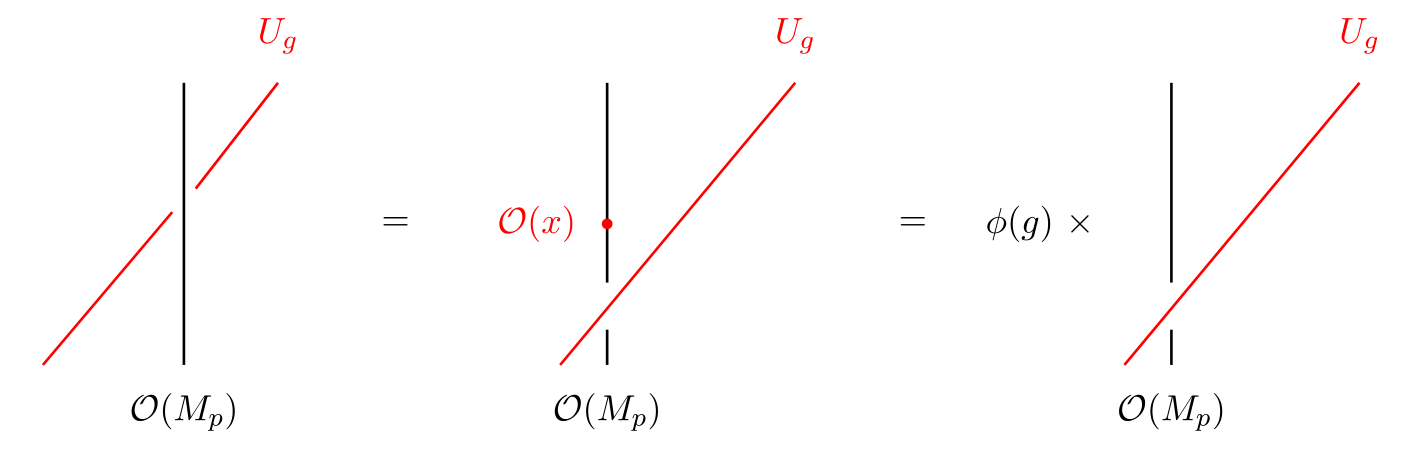
\includegraphics[scale=0.4]{figures/linking2.png}
	\caption{Taken from \cite{Bhardwaj}.} 
\end{figure}
The composition of the group induces a composition of those functions $\phi(g)$, 
\begin{equation}
	\phi(g)\phi(g')=\phi(gg').
\end{equation}
Therefore the functions $\phi(g)$ form a 1-dimensional representation of the $p$-form group $G^p$.  Since $G^p$ is an abelian group, from Schur’s Lemma we know that every irreducible representation of this group is 1-dimensional, then the functions $\phi(g)$ form precisely the irreducible representation of the group $G^p$. Therefore, the operators $\mathcal{O}(M_p)$ transforms under the fundamental representations of the $p$-form group, which shows that the charged objects under $p$-form symmetries are extended operators supported on $p$-dimensional manifolds. 

We can easily generalize the result we have seen before for the computation of the charge of the operator. For some  charged operator $\mathcal{O}(\Sigma_p)$ with charge $q\in\mathbb{Z}$ we have
\begin{equation}\label{action of hf symmetry}
	(d\star j)\mathcal{O}(\Sigma_D)=q\delta^{D-p}(\Sigma_p)\mathcal{O}(\Sigma_D)
\end{equation}
where $\delta^{D-p}(\Sigma_p)$  is the Poincaré dual of the delta function defined on $\Sigma_D$. Hence, for extended operators we have 
\begin{equation}
	U_g(S^{D-1})\mathcal{O}(\Sigma_p)=\exp(i\alpha q)\mathcal{O}(S^{D-1}).
\end{equation}
To summarize our results, let us study a $U(1)$ gauge theory in $D$ dimensions. 
\subsection*{U(1) Gauge Theory in $D$ dimensions}
Let $A$ be a 1-form $U(1)$ gauge field with 
\begin{equation}\label{conservation law maxwell}
	F=dA,
\end{equation}
where $F$ is a 2-form. In $D=4$, this is precisely Maxwell theory. From (\ref{conservation law maxwell}) we have
\begin{equation}
	dF=d\star(\star F)=0. 
\end{equation}
Therefore the Noether current then is the $(D-2)$-form, $\star F$.  The conserved charge is 
\begin{equation}
	Q^m=\int_{\Sigma_2}\star (\star F)=\int_{\Sigma_2}F,
\end{equation}
and the unitary operator is 
\begin{equation}
	U_g^m(\Sigma_2)=\exp\left(i\alpha\int_{\Sigma_2}F\right).
\end{equation}
The index $m$ appears because we call this the \textit{magnetic symmetry}. For $p\geq 1$-forms we integrate the charge over a $D-p-1$ manifold. Since this is 2-dimensional manifold, $D-p-1=2\Rightarrow p=D-3$. Thus, the magnetic symmetry is related to a $(D-3)$-form symmetry. 

The other conservation law follows from the ``Maxwell'' equations,
\begin{equation}
	d\star F=0,
\end{equation} 
which implies that in this case the conserved current is the 2-form, $F$. The conserved charge is 
\begin{equation}
	Q^e=\int_{D-2}\star F, 
\end{equation}
And the unitary operator
\begin{equation}
	U^e_g(\Sigma_{D-2})=\exp\left(i\alpha\int_{D-2}\star F\right).
\end{equation}
This is the \textit{electric symmetry}. In this case, $D-p-1=D-2\Rightarrow p=1$. Then, the electric symmetry is a 1-form symmetry, independent of the dimension. 

Therefore, this $U(1)$ gauge theory has 2 higher-form symmetries, an \textit{electric 1-form symmetry} and a \textit{magnetic $(D-3)$-form symmetry.} We represent then the symmetry group as 
\begin{equation}
	U(1)_e\times U(1)_m. 
\end{equation}
In $D=4$, the charged objects under the electric 1-form symmetry are the \textit{Wilson lines $W_q(L)$},
\begin{equation}
	W_q(L)=\exp\left(iq\int A_L\right),
\end{equation}
where $q$ is the charge of the Wilson line. Using (\ref{action of hf symmetry}) we have
\begin{equation}
	(d\star F)W_q(L)=q\delta^{D-1}(L)W_q(L). 
\end{equation}
This shows that the electric 1-form symmetry measures the charge of the Wilson line.

The charged objects under the magnetic $(D-3)$-form symmetry are the \textit{'t Hooft lines $T(\Sigma_{D-3})$.} Using the same idea, we can show that the magnetic $(D-3)$-form symmetry measures the magnetic charge of the 't Hooft line. 
\section{Discrete Gauge Symmetries}
Discrete gauge symmetries are related to symmetry transformations that belongs to discrete groups, rather continuous. It can be better understood in terms of higher-form symmetries. Before we understand how this works, we need to introduce two concepts, the \textit{Pontryagin dual} and the \textit{Screening} of operators. 

\subsection{Pontryagin Dual}
For some $p$-form symmetry group $G^{(p)}$ we may define the homomorphism 
\begin{equation}
	\phi:G^{(p)}\to U(1). 
\end{equation}
These maps form a group, 
\begin{equation}
	\phi(g)\phi'(g)=(\phi\phi')(g)\in U(1).
\end{equation}
We denote this group by 
\begin{equation}
	\widehat{G}^{(p)}=\{\text{all homomorphisms }G^{(p)}\to U(1) \}.
\end{equation}
Let us ilustrate this idea with two examples. 
\subsubsection*{Example: $G^{p}=U(1)$}
Define the homomorphism as,
\begin{equation}
	\phi(g)=g^q=e^{i\alpha q},\; \alpha\in [0,2\pi),\;q\in\mathbb{Z}.
\end{equation}
Let 
\begin{align}
	&\phi_1(g)=g,\\
	&\phi_2(g)=g^2\\
	&\phi_3(g)=g^3.
\end{align}
The composition gives, 
\begin{equation}
	\phi_1(g)\phi_2(g)=\phi_3(g). 
\end{equation}
This is the composition rule of the $\mathbb{Z}$ group. Therefore the Pontryagin dual for $U(1)$ is 
\begin{equation}
	\widehat{G}^{(p)}=\mathbb{Z}.
\end{equation}
\subsubsection*{Example: $G^{p}=\mathbb{Z}_N$}
In this case, $g=e^{\frac{2\pi i\alpha}{N}}$. Defining the homomorphism as 
\begin{equation}
	\phi=g^q=e^{\frac{2\pi i\alpha q}{N}}.
\end{equation}
Take $N=3$ and let 
\begin{align}
	&\phi_1(g)=g\\
	&\phi_2(g)=g^2. 
\end{align}
The composition gives 
\begin{equation}
	\phi_1(g)\phi_2(g)=\phi_1(g).
\end{equation}
Which is the composition rule of $\mathbb{Z}_N$. Therefore
\begin{equation}
	\widehat{G}^{(p)}=\mathbb{Z}_N.
\end{equation}
That is, the Pontryagin dual of $\mathbb{Z}_N$ is the group itself. 
\subsubsection*{Double Pontryagin Duality}
Since 
\begin{equation}
	\phi:G^{(p)}\to U(1),
\end{equation}
we can take 
\begin{equation}
	\varphi:\widehat{G}^{(p)}\to U(1). 
\end{equation}
Note that $\phi(g)\in U(1)$ and $\varphi(\phi(g))\in (1)$, then 
\begin{equation}
\widehat{\widehat{G}^{(p)}}=G^{(p)}.
\end{equation}

\subsection{Screening}
\begin{definition}
	A $p\geq 1$-dimensional operator $\mathcal{O}_p$ can be screened into another operator $\mathcal{O}'_p$ if there exists a $(p-1)$-dimensional operator $\mathcal{O}_{p-1}$ that can be inserted between $O_p$ and $O_p'$. 
	\begin{figure}[H]
		\centering
		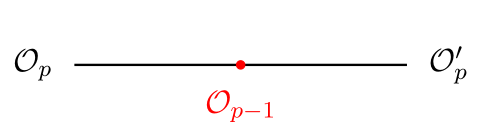
\includegraphics[scale=0.4]{figures/screening.png}
		\caption{Taken from \cite{Bhardwaj}.}
	\end{figure}
If $\mathcal{O}_p$ can be screened to the identity we say that it was completely screened. 
\end{definition}
\textit{Screening implies in the same charges.} Note that if two operators $\mathcal{O}_p$ and $\mathcal{O}'_p$ are screened, the symmetry operator 

\nocite{*}
\bibliography{refs.bib}
\bibliographystyle{ieeetr}
\end{document}
